\documentclass[1p]{elsarticle_modified}
%\bibliographystyle{elsarticle-num}

%\usepackage[colorlinks]{hyperref}
%\usepackage{abbrmath_seonhwa} %\Abb, \Ascr, \Acal ,\Abf, \Afrak
\usepackage{amsfonts}
\usepackage{amssymb}
\usepackage{amsmath}
\usepackage{amsthm}
\usepackage{scalefnt}
\usepackage{amsbsy}
\usepackage{kotex}
\usepackage{caption}
\usepackage{subfig}
\usepackage{color}
\usepackage{graphicx}
\usepackage{xcolor} %% white, black, red, green, blue, cyan, magenta, yellow
\usepackage{float}
\usepackage{setspace}
\usepackage{hyperref}

\usepackage{tikz}
\usetikzlibrary{arrows}

\usepackage{multirow}
\usepackage{array} % fixed length table
\usepackage{hhline}

%%%%%%%%%%%%%%%%%%%%%
\makeatletter
\renewcommand*\env@matrix[1][\arraystretch]{%
	\edef\arraystretch{#1}%
	\hskip -\arraycolsep
	\let\@ifnextchar\new@ifnextchar
	\array{*\c@MaxMatrixCols c}}
\makeatother %https://tex.stackexchange.com/questions/14071/how-can-i-increase-the-line-spacing-in-a-matrix
%%%%%%%%%%%%%%%

\usepackage[normalem]{ulem}

\newcommand{\msout}[1]{\ifmmode\text{\sout{\ensuremath{#1}}}\else\sout{#1}\fi}
%SOURCE: \msout is \stkout macro in https://tex.stackexchange.com/questions/20609/strikeout-in-math-mode

\newcommand{\cancel}[1]{
	\ifmmode
	{\color{red}\msout{#1}}
	\else
	{\color{red}\sout{#1}}
	\fi
}

\newcommand{\add}[1]{
	{\color{blue}\uwave{#1}}
}

\newcommand{\replace}[2]{
	\ifmmode
	{\color{red}\msout{#1}}{\color{blue}\uwave{#2}}
	\else
	{\color{red}\sout{#1}}{\color{blue}\uwave{#2}}
	\fi
}

\newcommand{\Sol}{\mathcal{S}} %segment
\newcommand{\D}{D} %diagram
\newcommand{\A}{\mathcal{A}} %arc


%%%%%%%%%%%%%%%%%%%%%%%%%%%%%5 test

\def\sl{\operatorname{\textup{SL}}(2,\Cbb)}
\def\psl{\operatorname{\textup{PSL}}(2,\Cbb)}
\def\quan{\mkern 1mu \triangleright \mkern 1mu}

\theoremstyle{definition}
\newtheorem{thm}{Theorem}[section]
\newtheorem{prop}[thm]{Proposition}
\newtheorem{lem}[thm]{Lemma}
\newtheorem{ques}[thm]{Question}
\newtheorem{cor}[thm]{Corollary}
\newtheorem{defn}[thm]{Definition}
\newtheorem{exam}[thm]{Example}
\newtheorem{rmk}[thm]{Remark}
\newtheorem{alg}[thm]{Algorithm}

\newcommand{\I}{\sqrt{-1}}
\begin{document}

%\begin{frontmatter}
%
%\title{Boundary parabolic representations of knots up to 8 crossings}
%
%%% Group authors per affiliation:
%\author{Yunhi Cho} 
%\address{Department of Mathematics, University of Seoul, Seoul, Korea}
%\ead{yhcho@uos.ac.kr}
%
%
%\author{Seonhwa Kim} %\fnref{s_kim}}
%\address{Center for Geometry and Physics, Institute for Basic Science, Pohang, 37673, Korea}
%\ead{ryeona17@ibs.re.kr}
%
%\author{Hyuk Kim}
%\address{Department of Mathematical Sciences, Seoul National University, Seoul 08826, Korea}
%\ead{hyukkim@snu.ac.kr}
%
%\author{Seokbeom Yoon}
%\address{Department of Mathematical Sciences, Seoul National University, Seoul, 08826,  Korea}
%\ead{sbyoon15@snu.ac.kr}
%
%\begin{abstract}
%We find all boundary parabolic representation of knots up to 8 crossings.
%
%\end{abstract}
%\begin{keyword}
%    \MSC[2010] 57M25 
%\end{keyword}
%
%\end{frontmatter}

%\linenumbers
%\tableofcontents
%
\newcommand\colored[1]{\textcolor{white}{\rule[-0.35ex]{0.8em}{1.4ex}}\kern-0.8em\color{red} #1}%
%\newcommand\colored[1]{\textcolor{white}{ #1}\kern-2.17ex	\textcolor{white}{ #1}\kern-1.81ex	\textcolor{white}{ #1}\kern-2.15ex\color{red}#1	}

{\Large $\underline{12n_{0880}~(K12n_{0880})}$}

\setlength{\tabcolsep}{10pt}
\renewcommand{\arraystretch}{1.6}
\vspace{1cm}\begin{tabular}{m{100pt}>{\centering\arraybackslash}m{274pt}}
\multirow{5}{120pt}{
	\centering
	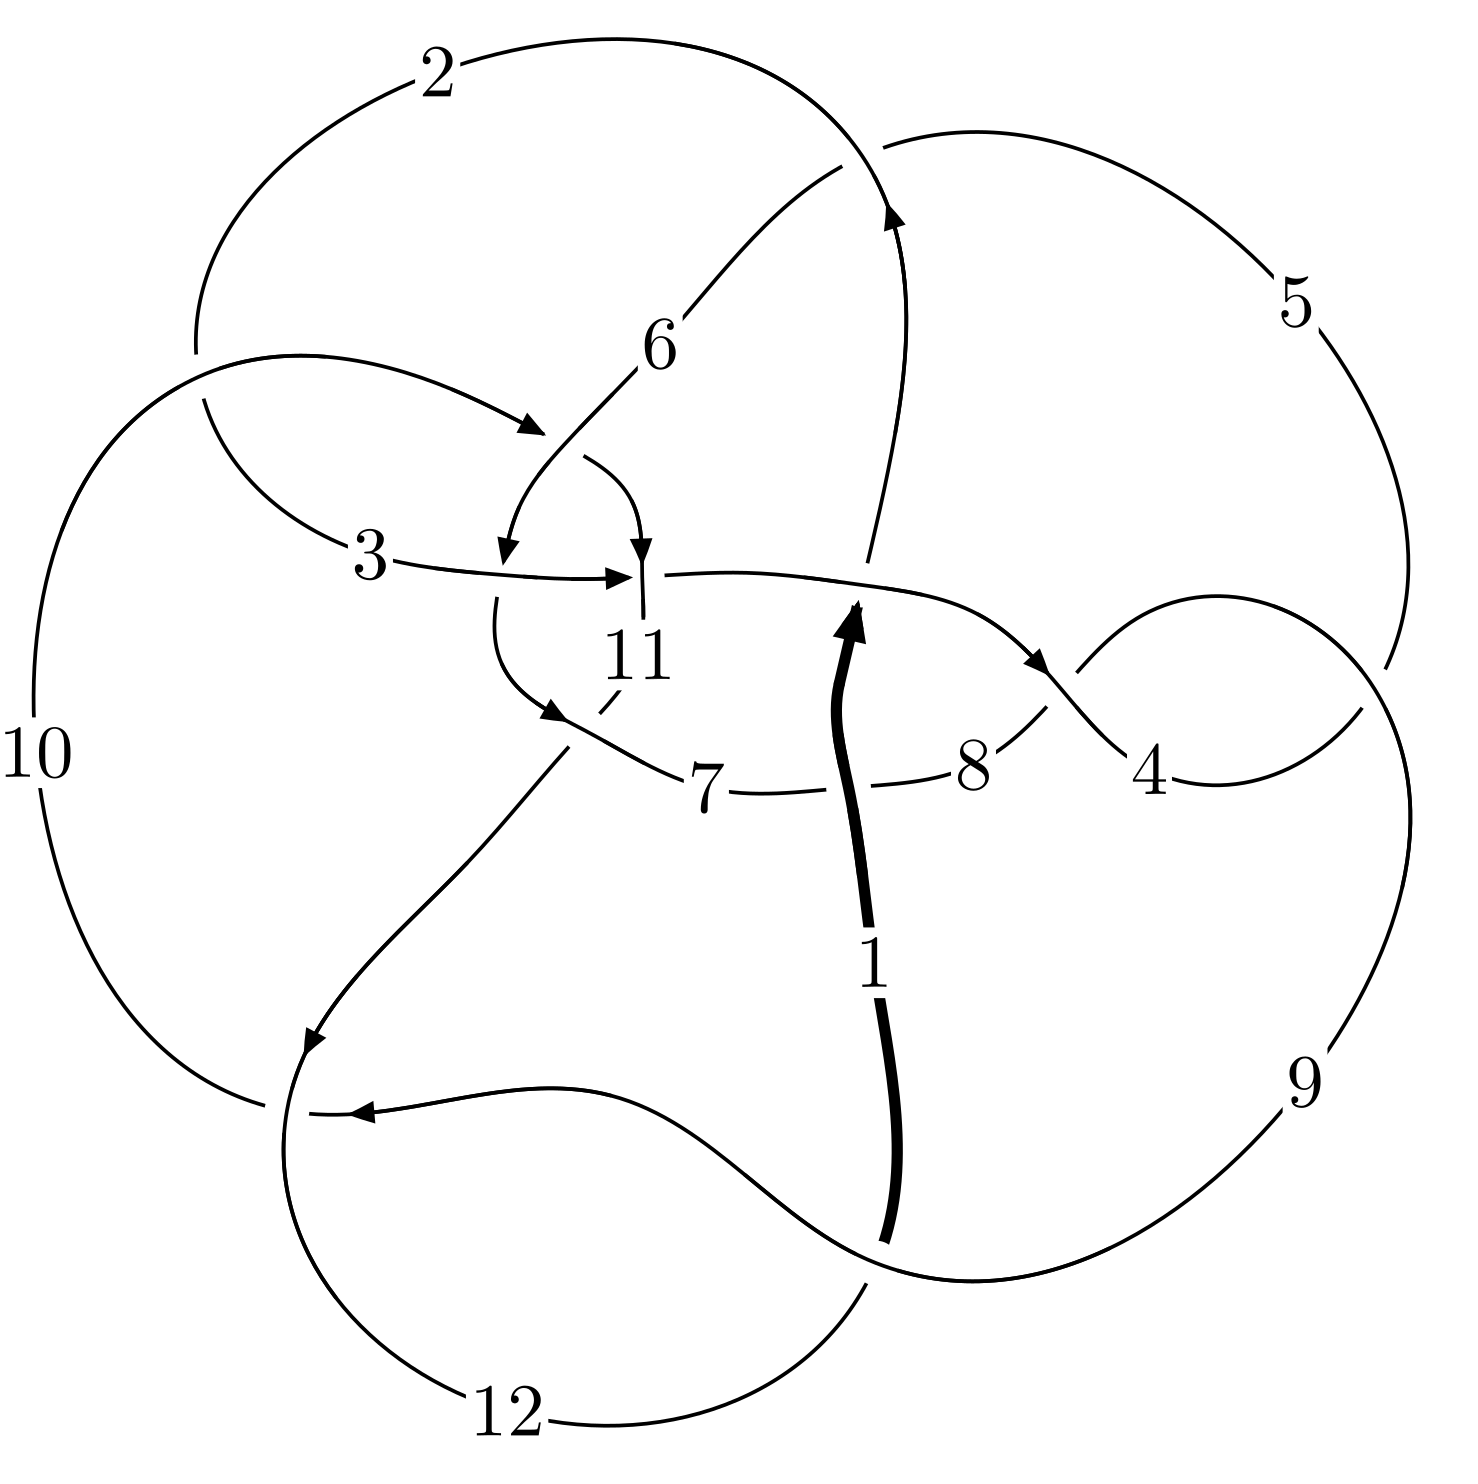
\includegraphics[width=112pt]{../../../GIT/diagram.site/Diagrams/png/2969_12n_0880.png}\\
\ \ \ A knot diagram\footnotemark}&
\allowdisplaybreaks
\textbf{Linearized knot diagam} \\
\cline{2-2}
 &
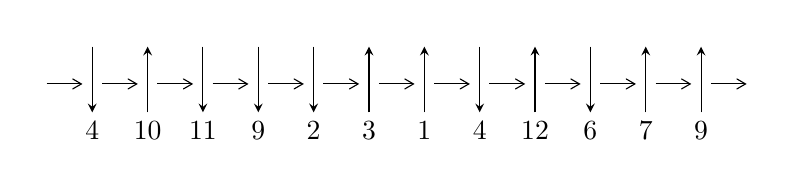
\begin{tikzpicture}[x=20pt, y=17pt]
	% nodes
	\node (C0) at (0, 0) {};
	\node (C1) at (1, 0) {};
	\node (C1U) at (1, +1) {};
	\node (C1D) at (1, -1) {4};

	\node (C2) at (2, 0) {};
	\node (C2U) at (2, +1) {};
	\node (C2D) at (2, -1) {10};

	\node (C3) at (3, 0) {};
	\node (C3U) at (3, +1) {};
	\node (C3D) at (3, -1) {11};

	\node (C4) at (4, 0) {};
	\node (C4U) at (4, +1) {};
	\node (C4D) at (4, -1) {9};

	\node (C5) at (5, 0) {};
	\node (C5U) at (5, +1) {};
	\node (C5D) at (5, -1) {2};

	\node (C6) at (6, 0) {};
	\node (C6U) at (6, +1) {};
	\node (C6D) at (6, -1) {3};

	\node (C7) at (7, 0) {};
	\node (C7U) at (7, +1) {};
	\node (C7D) at (7, -1) {1};

	\node (C8) at (8, 0) {};
	\node (C8U) at (8, +1) {};
	\node (C8D) at (8, -1) {4};

	\node (C9) at (9, 0) {};
	\node (C9U) at (9, +1) {};
	\node (C9D) at (9, -1) {12};

	\node (C10) at (10, 0) {};
	\node (C10U) at (10, +1) {};
	\node (C10D) at (10, -1) {6};

	\node (C11) at (11, 0) {};
	\node (C11U) at (11, +1) {};
	\node (C11D) at (11, -1) {7};

	\node (C12) at (12, 0) {};
	\node (C12U) at (12, +1) {};
	\node (C12D) at (12, -1) {9};
	\node (C13) at (13, 0) {};

	% arrows
	\draw[->,>={angle 60}]
	(C0) edge (C1) (C1) edge (C2) (C2) edge (C3) (C3) edge (C4) (C4) edge (C5) (C5) edge (C6) (C6) edge (C7) (C7) edge (C8) (C8) edge (C9) (C9) edge (C10) (C10) edge (C11) (C11) edge (C12) (C12) edge (C13) ;	\draw[->,>=stealth]
	(C1U) edge (C1D) (C2D) edge (C2U) (C3U) edge (C3D) (C4U) edge (C4D) (C5U) edge (C5D) (C6D) edge (C6U) (C7D) edge (C7U) (C8U) edge (C8D) (C9D) edge (C9U) (C10U) edge (C10D) (C11D) edge (C11U) (C12D) edge (C12U) ;
	\end{tikzpicture} \\
\hhline{~~} \\& 
\textbf{Solving Sequence} \\ \cline{2-2} 
 &
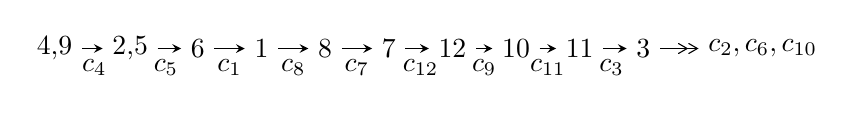
\begin{tikzpicture}[x=23pt, y=7pt]
	% node
	\node (A0) at (-1/8, 0) {4,9};
	\node (A1) at (17/16, 0) {2,5};
	\node (A2) at (17/8, 0) {6};
	\node (A3) at (25/8, 0) {1};
	\node (A4) at (33/8, 0) {8};
	\node (A5) at (41/8, 0) {7};
	\node (A6) at (49/8, 0) {12};
	\node (A7) at (57/8, 0) {10};
	\node (A8) at (65/8, 0) {11};
	\node (A9) at (73/8, 0) {3};
	\node (C1) at (1/2, -1) {$c_{4}$};
	\node (C2) at (13/8, -1) {$c_{5}$};
	\node (C3) at (21/8, -1) {$c_{1}$};
	\node (C4) at (29/8, -1) {$c_{8}$};
	\node (C5) at (37/8, -1) {$c_{7}$};
	\node (C6) at (45/8, -1) {$c_{12}$};
	\node (C7) at (53/8, -1) {$c_{9}$};
	\node (C8) at (61/8, -1) {$c_{11}$};
	\node (C9) at (69/8, -1) {$c_{3}$};
	\node (A10) at (11, 0) {$c_{2},c_{6},c_{10}$};

	% edge
	\draw[->,>=stealth]	
	(A0) edge (A1) (A1) edge (A2) (A2) edge (A3) (A3) edge (A4) (A4) edge (A5) (A5) edge (A6) (A6) edge (A7) (A7) edge (A8) (A8) edge (A9) ;
	\draw[->>,>={angle 60}]	
	(A9) edge (A10);
\end{tikzpicture} \\ 

\end{tabular} \\

\footnotetext{
The image of knot diagram is generated by the software ``\textbf{Draw programme}" developed by Andrew Bartholomew(\url{http://www.layer8.co.uk/maths/draw/index.htm\#Running-draw}), where we modified some parts for our purpose(\url{https://github.com/CATsTAILs/LinksPainter}).
}\phantom \\ \newline 
\centering \textbf{Ideals for irreducible components\footnotemark of $X_{\text{par}}$} 
 
\begin{align*}
I^u_{1}&=\langle 
b- u,\;-1.08548\times10^{25} u^{28}-9.54353\times10^{24} u^{27}+\cdots+2.18894\times10^{25} a-1.64519\times10^{26},\\
\phantom{I^u_{1}}&\phantom{= \langle  }u^{29}+2 u^{28}+\cdots-13 u^2-1\rangle \\
I^u_{2}&=\langle 
3.30161\times10^{299} u^{69}+1.46925\times10^{300} u^{68}+\cdots+1.12043\times10^{304} b+1.34425\times10^{304},\\
\phantom{I^u_{2}}&\phantom{= \langle  }9.23538\times10^{303} u^{69}+3.54679\times10^{304} u^{68}+\cdots+8.20265\times10^{307} a-3.71102\times10^{308},\\
\phantom{I^u_{2}}&\phantom{= \langle  }u^{70}+4 u^{69}+\cdots-25055 u+7321\rangle \\
I^u_{3}&=\langle 
b+u,\;559 u^{16}+807 u^{15}+\cdots+229 a-7206,\;u^{17}-2 u^{16}+\cdots+7 u-1\rangle \\
I^u_{4}&=\langle 
-33628 u^{15}+98620 u^{14}+\cdots+332531 b+154483,\\
\phantom{I^u_{4}}&\phantom{= \langle  }-311649 u^{15}+1539315 u^{14}+\cdots+332531 a-733442,\;u^{16}-5 u^{15}+\cdots- u+1\rangle \\
\\
\end{align*}
\raggedright * 4 irreducible components of $\dim_{\mathbb{C}}=0$, with total 132 representations.\\
\footnotetext{All coefficients of polynomials are rational numbers. But the coefficients are sometimes approximated in decimal forms when there is not enough margin.}
\newpage
\renewcommand{\arraystretch}{1}
\centering \section*{I. $I^u_{1}= \langle b- u,\;-1.09\times10^{25} u^{28}-9.54\times10^{24} u^{27}+\cdots+2.19\times10^{25} a-1.65\times10^{26},\;u^{29}+2 u^{28}+\cdots-13 u^2-1 \rangle$}
\flushleft \textbf{(i) Arc colorings}\\
\begin{tabular}{m{7pt} m{180pt} m{7pt} m{180pt} }
\flushright $a_{4}=$&$\begin{pmatrix}1\\0\end{pmatrix}$ \\
\flushright $a_{9}=$&$\begin{pmatrix}0\\u\end{pmatrix}$ \\
\flushright $a_{2}=$&$\begin{pmatrix}0.495891 u^{28}+0.435988 u^{27}+\cdots-9.79192 u+7.51592\\u\end{pmatrix}$ \\
\flushright $a_{5}=$&$\begin{pmatrix}1\\u^2\end{pmatrix}$ \\
\flushright $a_{6}=$&$\begin{pmatrix}-0.236452 u^{28}-0.866910 u^{27}+\cdots+0.968434 u+5.19398\\-0.00914076 u^{28}+0.0683031 u^{27}+\cdots+0.555793 u-0.105732\end{pmatrix}$ \\
\flushright $a_{1}=$&$\begin{pmatrix}0.495891 u^{28}+0.435988 u^{27}+\cdots-8.79192 u+7.51592\\u\end{pmatrix}$ \\
\flushright $a_{8}=$&$\begin{pmatrix}u\\u\end{pmatrix}$ \\
\flushright $a_{7}=$&$\begin{pmatrix}3.59236 u^{28}+7.49492 u^{27}+\cdots-29.5652 u-5.99169\\-0.105732 u^{28}-0.220604 u^{27}+\cdots+0.504109 u+0.555793\end{pmatrix}$ \\
\flushright $a_{12}=$&$\begin{pmatrix}0.495891 u^{28}+0.435988 u^{27}+\cdots-8.79192 u+7.51592\\0.105732 u^{28}+0.220604 u^{27}+\cdots+1.49589 u-0.555793\end{pmatrix}$ \\
\flushright $a_{10}=$&$\begin{pmatrix}-3.48663 u^{28}-7.27432 u^{27}+\cdots+31.0611 u+5.43590\\0.432299 u^{28}+0.854537 u^{27}+\cdots-1.99074 u-0.856852\end{pmatrix}$ \\
\flushright $a_{11}=$&$\begin{pmatrix}-4.79535 u^{28}-10.1485 u^{27}+\cdots+37.3810 u+9.72731\\0.567598 u^{28}+1.08259 u^{27}+\cdots-2.27410 u-0.965582\end{pmatrix}$ \\
\flushright $a_{3}=$&$\begin{pmatrix}-4.76966 u^{28}-9.82306 u^{27}+\cdots+37.4134 u+7.57843\\0.536273 u^{28}+1.28218 u^{27}+\cdots-3.23320 u-1.87683\end{pmatrix}$\\&\end{tabular}
\flushleft \textbf{(ii) Obstruction class $= -1$}\\~\\
\flushleft \textbf{(iii) Cusp Shapes $= -\frac{15517893495020098849975116}{21889407595733348190792803} u^{28}-\frac{54924211629619166277092344}{21889407595733348190792803} u^{27}+\cdots-\frac{191772394078626200464288803}{21889407595733348190792803} u+\frac{272223026286751222003122765}{21889407595733348190792803}$}\\~\\
\newpage\renewcommand{\arraystretch}{1}
\flushleft \textbf{(iv) u-Polynomials at the component}\newline \\
\begin{tabular}{m{50pt}|m{274pt}}
Crossings & \hspace{64pt}u-Polynomials at each crossing \\
\hline $$\begin{aligned}c_{1},c_{4},c_{8}\end{aligned}$$&$\begin{aligned}
&u^{29}+2 u^{28}+\cdots-13 u^2-1
\end{aligned}$\\
\hline $$\begin{aligned}c_{2},c_{11}\end{aligned}$$&$\begin{aligned}
&u^{29}- u^{28}+\cdots+6 u-1
\end{aligned}$\\
\hline $$\begin{aligned}c_{3},c_{10}\end{aligned}$$&$\begin{aligned}
&u^{29}- u^{28}+\cdots+3 u-1
\end{aligned}$\\
\hline $$\begin{aligned}c_{5}\end{aligned}$$&$\begin{aligned}
&u^{29}-2 u^{28}+\cdots+15 u-1
\end{aligned}$\\
\hline $$\begin{aligned}c_{6}\end{aligned}$$&$\begin{aligned}
&u^{29}-19 u^{28}+\cdots-36 u+8
\end{aligned}$\\
\hline $$\begin{aligned}c_{7}\end{aligned}$$&$\begin{aligned}
&u^{29}-25 u^{28}+\cdots+26368 u-2560
\end{aligned}$\\
\hline $$\begin{aligned}c_{9},c_{12}\end{aligned}$$&$\begin{aligned}
&u^{29}+13 u^{28}+\cdots-544 u-64
\end{aligned}$\\
\hline
\end{tabular}\\~\\
\newpage\renewcommand{\arraystretch}{1}
\flushleft \textbf{(v) Riley Polynomials at the component}\newline \\
\begin{tabular}{m{50pt}|m{274pt}}
Crossings & \hspace{64pt}Riley Polynomials at each crossing \\
\hline $$\begin{aligned}c_{1},c_{4},c_{8}\end{aligned}$$&$\begin{aligned}
&y^{29}+38 y^{28}+\cdots-26 y-1
\end{aligned}$\\
\hline $$\begin{aligned}c_{2},c_{11}\end{aligned}$$&$\begin{aligned}
&y^{29}-3 y^{28}+\cdots+8 y-1
\end{aligned}$\\
\hline $$\begin{aligned}c_{3},c_{10}\end{aligned}$$&$\begin{aligned}
&y^{29}-7 y^{28}+\cdots+11 y-1
\end{aligned}$\\
\hline $$\begin{aligned}c_{5}\end{aligned}$$&$\begin{aligned}
&y^{29}+2 y^{28}+\cdots+99 y-1
\end{aligned}$\\
\hline $$\begin{aligned}c_{6}\end{aligned}$$&$\begin{aligned}
&y^{29}+3 y^{28}+\cdots-1264 y-64
\end{aligned}$\\
\hline $$\begin{aligned}c_{7}\end{aligned}$$&$\begin{aligned}
&y^{29}-17 y^{28}+\cdots-26279936 y-6553600
\end{aligned}$\\
\hline $$\begin{aligned}c_{9},c_{12}\end{aligned}$$&$\begin{aligned}
&y^{29}+17 y^{28}+\cdots-52736 y-4096
\end{aligned}$\\
\hline
\end{tabular}\\~\\
\newpage\flushleft \textbf{(vi) Complex Volumes and Cusp Shapes}
$$\begin{array}{c|c|c}  
\text{Solutions to }I^u_{1}& \I (\text{vol} + \sqrt{-1}CS) & \text{Cusp shape}\\
 \hline 
\begin{aligned}
u &= -0.642235 + 0.726664 I \\
a &= -0.949259 + 0.155912 I \\
b &= -0.642235 + 0.726664 I\end{aligned}
 & -3.06174 - 3.25839 I & -7.69069 + 6.26564 I \\ \hline\begin{aligned}
u &= -0.642235 - 0.726664 I \\
a &= -0.949259 - 0.155912 I \\
b &= -0.642235 - 0.726664 I\end{aligned}
 & -3.06174 + 3.25839 I & -7.69069 - 6.26564 I \\ \hline\begin{aligned}
u &= -0.032170 + 0.801563 I \\
a &= \phantom{-}1.55712 - 0.56759 I \\
b &= -0.032170 + 0.801563 I\end{aligned}
 & -0.504140 + 0.951000 I & \phantom{-}1.54358 - 2.27904 I \\ \hline\begin{aligned}
u &= -0.032170 - 0.801563 I \\
a &= \phantom{-}1.55712 + 0.56759 I \\
b &= -0.032170 - 0.801563 I\end{aligned}
 & -0.504140 - 0.951000 I & \phantom{-}1.54358 + 2.27904 I \\ \hline\begin{aligned}
u &= \phantom{-}0.198126 + 0.740818 I \\
a &= -0.655188 + 0.248714 I \\
b &= \phantom{-}0.198126 + 0.740818 I\end{aligned}
 & \phantom{-}2.37624 + 4.78664 I & \phantom{-}2.73963 - 5.44891 I \\ \hline\begin{aligned}
u &= \phantom{-}0.198126 - 0.740818 I \\
a &= -0.655188 - 0.248714 I \\
b &= \phantom{-}0.198126 - 0.740818 I\end{aligned}
 & \phantom{-}2.37624 - 4.78664 I & \phantom{-}2.73963 + 5.44891 I \\ \hline\begin{aligned}
u &= -0.661536 + 0.319149 I \\
a &= \phantom{-}1.41580 - 1.68650 I \\
b &= -0.661536 + 0.319149 I\end{aligned}
 & -4.19456 + 0.95591 I & -0.74396 - 10.67777 I \\ \hline\begin{aligned}
u &= -0.661536 - 0.319149 I \\
a &= \phantom{-}1.41580 + 1.68650 I \\
b &= -0.661536 - 0.319149 I\end{aligned}
 & -4.19456 - 0.95591 I & -0.74396 + 10.67777 I \\ \hline\begin{aligned}
u &= \phantom{-}0.363420 + 0.611313 I \\
a &= -2.25022 - 1.12399 I \\
b &= \phantom{-}0.363420 + 0.611313 I\end{aligned}
 & -2.25137 + 9.11530 I & \phantom{-}0.91619 - 5.98946 I \\ \hline\begin{aligned}
u &= \phantom{-}0.363420 - 0.611313 I \\
a &= -2.25022 + 1.12399 I \\
b &= \phantom{-}0.363420 - 0.611313 I\end{aligned}
 & -2.25137 - 9.11530 I & \phantom{-}0.91619 + 5.98946 I\\
 \hline 
 \end{array}$$\newpage$$\begin{array}{c|c|c}  
\text{Solutions to }I^u_{1}& \I (\text{vol} + \sqrt{-1}CS) & \text{Cusp shape}\\
 \hline 
\begin{aligned}
u &= -0.36313 + 1.47042 I \\
a &= \phantom{-}0.008827 - 1.188710 I \\
b &= -0.36313 + 1.47042 I\end{aligned}
 & \phantom{-}2.73712 + 3.34248 I & -3.35900 - 2.79422 I \\ \hline\begin{aligned}
u &= -0.36313 - 1.47042 I \\
a &= \phantom{-}0.008827 + 1.188710 I \\
b &= -0.36313 - 1.47042 I\end{aligned}
 & \phantom{-}2.73712 - 3.34248 I & -3.35900 + 2.79422 I \\ \hline\begin{aligned}
u &= -0.064814 + 0.477187 I \\
a &= \phantom{-}1.022190 - 0.598774 I \\
b &= -0.064814 + 0.477187 I\end{aligned}
 & \phantom{-}0.008337 + 1.334080 I & \phantom{-}0.34791 - 4.25043 I \\ \hline\begin{aligned}
u &= -0.064814 - 0.477187 I \\
a &= \phantom{-}1.022190 + 0.598774 I \\
b &= -0.064814 - 0.477187 I\end{aligned}
 & \phantom{-}0.008337 - 1.334080 I & \phantom{-}0.34791 + 4.25043 I \\ \hline\begin{aligned}
u &= \phantom{-}0.44900 + 1.45880 I \\
a &= \phantom{-}0.178143 - 0.845770 I \\
b &= \phantom{-}0.44900 + 1.45880 I\end{aligned}
 & -0.088337 - 0.453344 I & -3.53660 + 0. I\phantom{ +0.000000I} \\ \hline\begin{aligned}
u &= \phantom{-}0.44900 - 1.45880 I \\
a &= \phantom{-}0.178143 + 0.845770 I \\
b &= \phantom{-}0.44900 - 1.45880 I\end{aligned}
 & -0.088337 + 0.453344 I & -3.53660 + 0. I\phantom{ +0.000000I} \\ \hline\begin{aligned}
u &= -0.42651 + 1.53556 I \\
a &= \phantom{-}0.063635 - 0.740740 I \\
b &= -0.42651 + 1.53556 I\end{aligned}
 & \phantom{-}1.85990 + 6.10163 I & \phantom{-0.000000 } 0. - 6.71936 I \\ \hline\begin{aligned}
u &= -0.42651 - 1.53556 I \\
a &= \phantom{-}0.063635 + 0.740740 I \\
b &= -0.42651 - 1.53556 I\end{aligned}
 & \phantom{-}1.85990 - 6.10163 I & \phantom{-0.000000 -}0. + 6.71936 I \\ \hline\begin{aligned}
u &= -0.00700 + 1.64434 I \\
a &= \phantom{-}0.387864 - 1.087010 I \\
b &= -0.00700 + 1.64434 I\end{aligned}
 & \phantom{-}5.36503 + 3.15379 I & \phantom{-0.000000 } 0. - 5.21676 I \\ \hline\begin{aligned}
u &= -0.00700 - 1.64434 I \\
a &= \phantom{-}0.387864 + 1.087010 I \\
b &= -0.00700 - 1.64434 I\end{aligned}
 & \phantom{-}5.36503 - 3.15379 I & \phantom{-0.000000 -}0. + 5.21676 I\\
 \hline 
 \end{array}$$\newpage$$\begin{array}{c|c|c}  
\text{Solutions to }I^u_{1}& \I (\text{vol} + \sqrt{-1}CS) & \text{Cusp shape}\\
 \hline 
\begin{aligned}
u &= -0.035016 + 0.329660 I \\
a &= \phantom{-}3.92347 - 1.51601 I \\
b &= -0.035016 + 0.329660 I\end{aligned}
 & -2.64525 + 3.58389 I & \phantom{-}5.38204 - 3.13101 I \\ \hline\begin{aligned}
u &= -0.035016 - 0.329660 I \\
a &= \phantom{-}3.92347 + 1.51601 I \\
b &= -0.035016 - 0.329660 I\end{aligned}
 & -2.64525 - 3.58389 I & \phantom{-}5.38204 + 3.13101 I \\ \hline\begin{aligned}
u &= \phantom{-}0.308534\phantom{ +0.000000I} \\
a &= \phantom{-}2.18209\phantom{ +0.000000I} \\
b &= \phantom{-}0.308534\phantom{ +0.000000I}\end{aligned}
 & \phantom{-}1.77894\phantom{ +0.000000I} & \phantom{-}6.13630\phantom{ +0.000000I} \\ \hline\begin{aligned}
u &= \phantom{-}0.02951 + 1.77011 I \\
a &= -0.345581 - 0.914758 I \\
b &= \phantom{-}0.02951 + 1.77011 I\end{aligned}
 & \phantom{-}7.48152 - 10.06130 I & \phantom{-0.000000 } 0 \\ \hline\begin{aligned}
u &= \phantom{-}0.02951 - 1.77011 I \\
a &= -0.345581 + 0.914758 I \\
b &= \phantom{-}0.02951 - 1.77011 I\end{aligned}
 & \phantom{-}7.48152 + 10.06130 I & \phantom{-0.000000 } 0 \\ \hline\begin{aligned}
u &= -0.52214 + 1.75074 I \\
a &= \phantom{-}0.049722 - 1.179220 I \\
b &= -0.52214 + 1.75074 I\end{aligned}
 & \phantom{-}3.80541 + 9.37886 I & \phantom{-0.000000 } 0 \\ \hline\begin{aligned}
u &= -0.52214 - 1.75074 I \\
a &= \phantom{-}0.049722 + 1.179220 I \\
b &= -0.52214 - 1.75074 I\end{aligned}
 & \phantom{-}3.80541 - 9.37886 I & \phantom{-0.000000 } 0 \\ \hline\begin{aligned}
u &= \phantom{-}0.56023 + 1.75971 I \\
a &= \phantom{-}0.002425 - 1.091640 I \\
b &= \phantom{-}0.56023 + 1.75971 I\end{aligned}
 & \phantom{-}4.6717 - 18.2246 I & \phantom{-0.000000 } 0 \\ \hline\begin{aligned}
u &= \phantom{-}0.56023 - 1.75971 I \\
a &= \phantom{-}0.002425 + 1.091640 I \\
b &= \phantom{-}0.56023 - 1.75971 I\end{aligned}
 & \phantom{-}4.6717 + 18.2246 I & \phantom{-0.000000 } 0\\
 \hline 
 \end{array}$$\newpage\newpage\renewcommand{\arraystretch}{1}
\centering \section*{II. $I^u_{2}= \langle 3.30\times10^{299} u^{69}+1.47\times10^{300} u^{68}+\cdots+1.12\times10^{304} b+1.34\times10^{304},\;9.24\times10^{303} u^{69}+3.55\times10^{304} u^{68}+\cdots+8.20\times10^{307} a-3.71\times10^{308},\;u^{70}+4 u^{69}+\cdots-25055 u+7321 \rangle$}
\flushleft \textbf{(i) Arc colorings}\\
\begin{tabular}{m{7pt} m{180pt} m{7pt} m{180pt} }
\flushright $a_{4}=$&$\begin{pmatrix}1\\0\end{pmatrix}$ \\
\flushright $a_{9}=$&$\begin{pmatrix}0\\u\end{pmatrix}$ \\
\flushright $a_{2}=$&$\begin{pmatrix}-0.000112590 u^{69}-0.000432396 u^{68}+\cdots+39.3655 u+4.52418\\-0.0000294674 u^{69}-0.000131133 u^{68}+\cdots+10.9533 u-1.19976\end{pmatrix}$ \\
\flushright $a_{5}=$&$\begin{pmatrix}1\\u^2\end{pmatrix}$ \\
\flushright $a_{6}=$&$\begin{pmatrix}-0.000220172 u^{69}-0.000838330 u^{68}+\cdots+22.3863 u+3.16969\\0.000123302 u^{69}+0.000461935 u^{68}+\cdots-0.298297 u+1.15154\end{pmatrix}$ \\
\flushright $a_{1}=$&$\begin{pmatrix}-0.000142058 u^{69}-0.000563529 u^{68}+\cdots+50.3188 u+3.32441\\-0.0000294674 u^{69}-0.000131133 u^{68}+\cdots+10.9533 u-1.19976\end{pmatrix}$ \\
\flushright $a_{8}=$&$\begin{pmatrix}u\\u\end{pmatrix}$ \\
\flushright $a_{7}=$&$\begin{pmatrix}-0.0000101216 u^{69}-0.000129726 u^{68}+\cdots-18.3646 u-6.84743\\8.90333\times10^{-6} u^{69}+0.0000205847 u^{68}+\cdots+2.62665 u-1.06858\end{pmatrix}$ \\
\flushright $a_{12}=$&$\begin{pmatrix}-0.000142058 u^{69}-0.000563529 u^{68}+\cdots+50.3188 u+3.32441\\2.71889\times10^{-6} u^{69}-0.0000339701 u^{68}+\cdots+12.1111 u-1.23418\end{pmatrix}$ \\
\flushright $a_{10}=$&$\begin{pmatrix}-0.0000424653 u^{69}-0.0000800391 u^{68}+\cdots+22.4206 u+6.90329\\-0.000106669 u^{69}-0.000435892 u^{68}+\cdots+6.61734 u-0.601728\end{pmatrix}$ \\
\flushright $a_{11}=$&$\begin{pmatrix}-0.000135005 u^{69}-0.000501852 u^{68}+\cdots-2.82311 u-1.87464\\0.0000112497 u^{69}-0.0000185942 u^{68}+\cdots+9.85186 u-1.86309\end{pmatrix}$ \\
\flushright $a_{3}=$&$\begin{pmatrix}0.0000677057 u^{69}+0.000381037 u^{68}+\cdots-9.38177 u+4.29494\\-0.000159969 u^{69}-0.000628642 u^{68}+\cdots+1.07104 u-0.793122\end{pmatrix}$\\&\end{tabular}
\flushleft \textbf{(ii) Obstruction class $= -1$}\\~\\
\flushleft \textbf{(iii) Cusp Shapes $= -0.000428326 u^{69}-0.00153541 u^{68}+\cdots+42.7410 u+1.53991$}\\~\\
\newpage\renewcommand{\arraystretch}{1}
\flushleft \textbf{(iv) u-Polynomials at the component}\newline \\
\begin{tabular}{m{50pt}|m{274pt}}
Crossings & \hspace{64pt}u-Polynomials at each crossing \\
\hline $$\begin{aligned}c_{1},c_{4},c_{8}\end{aligned}$$&$\begin{aligned}
&u^{70}+4 u^{69}+\cdots-25055 u+7321
\end{aligned}$\\
\hline $$\begin{aligned}c_{2},c_{11}\end{aligned}$$&$\begin{aligned}
&u^{70}+3 u^{69}+\cdots+4797 u+373
\end{aligned}$\\
\hline $$\begin{aligned}c_{3},c_{10}\end{aligned}$$&$\begin{aligned}
&u^{70}+7 u^{68}+\cdots-28 u+1
\end{aligned}$\\
\hline $$\begin{aligned}c_{5}\end{aligned}$$&$\begin{aligned}
&u^{70}+3 u^{69}+\cdots+13827 u-2381
\end{aligned}$\\
\hline $$\begin{aligned}c_{6}\end{aligned}$$&$\begin{aligned}
&(u^{35}+8 u^{34}+\cdots+4 u+1)^{2}
\end{aligned}$\\
\hline $$\begin{aligned}c_{7}\end{aligned}$$&$\begin{aligned}
&(u^{35}+13 u^{34}+\cdots-28 u-1)^{2}
\end{aligned}$\\
\hline $$\begin{aligned}c_{9},c_{12}\end{aligned}$$&$\begin{aligned}
&(u^{35}-10 u^{34}+\cdots+29 u-7)^{2}
\end{aligned}$\\
\hline
\end{tabular}\\~\\
\newpage\renewcommand{\arraystretch}{1}
\flushleft \textbf{(v) Riley Polynomials at the component}\newline \\
\begin{tabular}{m{50pt}|m{274pt}}
Crossings & \hspace{64pt}Riley Polynomials at each crossing \\
\hline $$\begin{aligned}c_{1},c_{4},c_{8}\end{aligned}$$&$\begin{aligned}
&y^{70}+64 y^{69}+\cdots-6291205415 y+53597041
\end{aligned}$\\
\hline $$\begin{aligned}c_{2},c_{11}\end{aligned}$$&$\begin{aligned}
&y^{70}- y^{69}+\cdots-4085189 y+139129
\end{aligned}$\\
\hline $$\begin{aligned}c_{3},c_{10}\end{aligned}$$&$\begin{aligned}
&y^{70}+14 y^{69}+\cdots-416 y+1
\end{aligned}$\\
\hline $$\begin{aligned}c_{5}\end{aligned}$$&$\begin{aligned}
&y^{70}+19 y^{69}+\cdots-521935401 y+5669161
\end{aligned}$\\
\hline $$\begin{aligned}c_{6}\end{aligned}$$&$\begin{aligned}
&(y^{35}-2 y^{34}+\cdots+18 y-1)^{2}
\end{aligned}$\\
\hline $$\begin{aligned}c_{7}\end{aligned}$$&$\begin{aligned}
&(y^{35}-45 y^{34}+\cdots+92 y-1)^{2}
\end{aligned}$\\
\hline $$\begin{aligned}c_{9},c_{12}\end{aligned}$$&$\begin{aligned}
&(y^{35}+12 y^{34}+\cdots-825 y-49)^{2}
\end{aligned}$\\
\hline
\end{tabular}\\~\\
\newpage\flushleft \textbf{(vi) Complex Volumes and Cusp Shapes}
$$\begin{array}{c|c|c}  
\text{Solutions to }I^u_{2}& \I (\text{vol} + \sqrt{-1}CS) & \text{Cusp shape}\\
 \hline 
\begin{aligned}
u &= \phantom{-}1.058400 + 0.079730 I \\
a &= \phantom{-}0.545962 + 0.044088 I \\
b &= \phantom{-}0.173597 + 0.712167 I\end{aligned}
 & \phantom{-}0.26528 + 2.69707 I & \phantom{-}5.39503 - 6.85723 I \\ \hline\begin{aligned}
u &= \phantom{-}1.058400 - 0.079730 I \\
a &= \phantom{-}0.545962 - 0.044088 I \\
b &= \phantom{-}0.173597 - 0.712167 I\end{aligned}
 & \phantom{-}0.26528 - 2.69707 I & \phantom{-}5.39503 + 6.85723 I \\ \hline\begin{aligned}
u &= -0.024911 + 0.911364 I \\
a &= \phantom{-}0.715176 - 0.576738 I \\
b &= -1.51437 + 0.36342 I\end{aligned}
 & -2.44566 - 0.09156 I & -4.00202 - 0.79327 I \\ \hline\begin{aligned}
u &= -0.024911 - 0.911364 I \\
a &= \phantom{-}0.715176 + 0.576738 I \\
b &= -1.51437 - 0.36342 I\end{aligned}
 & -2.44566 + 0.09156 I & -4.00202 + 0.79327 I \\ \hline\begin{aligned}
u &= -0.842982 + 0.298449 I \\
a &= -0.21865 + 1.68444 I \\
b &= -0.352984 - 0.459182 I\end{aligned}
 & -4.03807 - 1.26323 I & -2.43296 + 8.36038 I \\ \hline\begin{aligned}
u &= -0.842982 - 0.298449 I \\
a &= -0.21865 - 1.68444 I \\
b &= -0.352984 + 0.459182 I\end{aligned}
 & -4.03807 + 1.26323 I & -2.43296 - 8.36038 I \\ \hline\begin{aligned}
u &= -0.106910 + 1.108100 I \\
a &= \phantom{-}0.42598 + 1.51358 I \\
b &= -0.02176 - 1.91547 I\end{aligned}
 & \phantom{-}5.12124 - 4.17998 I & \phantom{-0.000000 } 0 \\ \hline\begin{aligned}
u &= -0.106910 - 1.108100 I \\
a &= \phantom{-}0.42598 - 1.51358 I \\
b &= -0.02176 + 1.91547 I\end{aligned}
 & \phantom{-}5.12124 + 4.17998 I & \phantom{-0.000000 } 0 \\ \hline\begin{aligned}
u &= -0.345458 + 0.796183 I \\
a &= \phantom{-}0.0813893 + 0.0438662 I \\
b &= -1.279940 - 0.228114 I\end{aligned}
 & -1.55070 - 2.22046 I & \phantom{-}3.51989 + 4.80032 I \\ \hline\begin{aligned}
u &= -0.345458 - 0.796183 I \\
a &= \phantom{-}0.0813893 - 0.0438662 I \\
b &= -1.279940 + 0.228114 I\end{aligned}
 & -1.55070 + 2.22046 I & \phantom{-}3.51989 - 4.80032 I\\
 \hline 
 \end{array}$$\newpage$$\begin{array}{c|c|c}  
\text{Solutions to }I^u_{2}& \I (\text{vol} + \sqrt{-1}CS) & \text{Cusp shape}\\
 \hline 
\begin{aligned}
u &= -0.332881 + 0.736341 I \\
a &= \phantom{-}0.809113 + 0.578377 I \\
b &= -1.332510 + 0.087336 I\end{aligned}
 & -2.58048 + 2.08849 I & -4.91472 - 12.36677 I \\ \hline\begin{aligned}
u &= -0.332881 - 0.736341 I \\
a &= \phantom{-}0.809113 - 0.578377 I \\
b &= -1.332510 - 0.087336 I\end{aligned}
 & -2.58048 - 2.08849 I & -4.91472 + 12.36677 I \\ \hline\begin{aligned}
u &= \phantom{-}0.771829\phantom{ +0.000000I} \\
a &= \phantom{-}1.06093\phantom{ +0.000000I} \\
b &= \phantom{-}0.0837624\phantom{ +0.000000I}\end{aligned}
 & \phantom{-}1.61445\phantom{ +0.000000I} & \phantom{-}9.96300\phantom{ +0.000000I} \\ \hline\begin{aligned}
u &= -0.198870 + 0.719238 I \\
a &= \phantom{-}0.841225 - 0.931153 I \\
b &= \phantom{-}0.715177 + 0.075240 I\end{aligned}
 & -2.56135 + 4.30729 I & -4.11547 - 11.98740 I \\ \hline\begin{aligned}
u &= -0.198870 - 0.719238 I \\
a &= \phantom{-}0.841225 + 0.931153 I \\
b &= \phantom{-}0.715177 - 0.075240 I\end{aligned}
 & -2.56135 - 4.30729 I & -4.11547 + 11.98740 I \\ \hline\begin{aligned}
u &= \phantom{-}0.173597 + 0.712167 I \\
a &= \phantom{-}0.305095 - 0.732082 I \\
b &= \phantom{-}1.058400 + 0.079730 I\end{aligned}
 & \phantom{-}0.26528 + 2.69707 I & \phantom{-}5.39503 - 6.85723 I \\ \hline\begin{aligned}
u &= \phantom{-}0.173597 - 0.712167 I \\
a &= \phantom{-}0.305095 + 0.732082 I \\
b &= \phantom{-}1.058400 - 0.079730 I\end{aligned}
 & \phantom{-}0.26528 - 2.69707 I & \phantom{-}5.39503 + 6.85723 I \\ \hline\begin{aligned}
u &= \phantom{-}0.715177 + 0.075240 I \\
a &= \phantom{-}0.809801 + 1.019730 I \\
b &= -0.198870 + 0.719238 I\end{aligned}
 & -2.56135 + 4.30729 I & -4.11547 - 11.98740 I \\ \hline\begin{aligned}
u &= \phantom{-}0.715177 - 0.075240 I \\
a &= \phantom{-}0.809801 - 1.019730 I \\
b &= -0.198870 - 0.719238 I\end{aligned}
 & -2.56135 - 4.30729 I & -4.11547 + 11.98740 I \\ \hline\begin{aligned}
u &= \phantom{-}0.030698 + 0.717655 I \\
a &= -0.490991 + 0.799569 I \\
b &= \phantom{-}1.56053 + 0.16062 I\end{aligned}
 & -1.79291 - 10.37620 I & \phantom{-}1.00185 + 8.04577 I\\
 \hline 
 \end{array}$$\newpage$$\begin{array}{c|c|c}  
\text{Solutions to }I^u_{2}& \I (\text{vol} + \sqrt{-1}CS) & \text{Cusp shape}\\
 \hline 
\begin{aligned}
u &= \phantom{-}0.030698 - 0.717655 I \\
a &= -0.490991 - 0.799569 I \\
b &= \phantom{-}1.56053 - 0.16062 I\end{aligned}
 & -1.79291 + 10.37620 I & \phantom{-}1.00185 - 8.04577 I \\ \hline\begin{aligned}
u &= -1.255260 + 0.308189 I \\
a &= \phantom{-}0.398382 - 0.072693 I \\
b &= -0.165206 - 0.197590 I\end{aligned}
 & -2.66687 + 0.36120 I & \phantom{-0.000000 } 0 \\ \hline\begin{aligned}
u &= -1.255260 - 0.308189 I \\
a &= \phantom{-}0.398382 + 0.072693 I \\
b &= -0.165206 + 0.197590 I\end{aligned}
 & -2.66687 - 0.36120 I & \phantom{-0.000000 } 0 \\ \hline\begin{aligned}
u &= -1.279940 + 0.228114 I \\
a &= \phantom{-}0.0410374 + 0.0461021 I \\
b &= -0.345458 - 0.796183 I\end{aligned}
 & -1.55070 + 2.22046 I & \phantom{-0.000000 } 0 \\ \hline\begin{aligned}
u &= -1.279940 - 0.228114 I \\
a &= \phantom{-}0.0410374 - 0.0461021 I \\
b &= -0.345458 + 0.796183 I\end{aligned}
 & -1.55070 - 2.22046 I & \phantom{-0.000000 } 0 \\ \hline\begin{aligned}
u &= \phantom{-}1.132590 + 0.686893 I \\
a &= -0.601873 - 0.054832 I \\
b &= -0.134777 - 0.571016 I\end{aligned}
 & -3.12149 - 5.64463 I & \phantom{-0.000000 } 0 \\ \hline\begin{aligned}
u &= \phantom{-}1.132590 - 0.686893 I \\
a &= -0.601873 + 0.054832 I \\
b &= -0.134777 + 0.571016 I\end{aligned}
 & -3.12149 + 5.64463 I & \phantom{-0.000000 } 0 \\ \hline\begin{aligned}
u &= -1.332510 + 0.087336 I \\
a &= \phantom{-}0.539255 - 0.267281 I \\
b &= -0.332881 + 0.736341 I\end{aligned}
 & -2.58048 + 2.08849 I & \phantom{-0.000000 } 0 \\ \hline\begin{aligned}
u &= -1.332510 - 0.087336 I \\
a &= \phantom{-}0.539255 + 0.267281 I \\
b &= -0.332881 - 0.736341 I\end{aligned}
 & -2.58048 - 2.08849 I & \phantom{-0.000000 } 0 \\ \hline\begin{aligned}
u &= \phantom{-}0.355920 + 1.345040 I \\
a &= -0.593513 + 0.907048 I \\
b &= \phantom{-}0.02059 - 1.72427 I\end{aligned}
 & \phantom{-}5.20790 - 1.91522 I & \phantom{-0.000000 } 0\\
 \hline 
 \end{array}$$\newpage$$\begin{array}{c|c|c}  
\text{Solutions to }I^u_{2}& \I (\text{vol} + \sqrt{-1}CS) & \text{Cusp shape}\\
 \hline 
\begin{aligned}
u &= \phantom{-}0.355920 - 1.345040 I \\
a &= -0.593513 - 0.907048 I \\
b &= \phantom{-}0.02059 + 1.72427 I\end{aligned}
 & \phantom{-}5.20790 + 1.91522 I & \phantom{-0.000000 } 0 \\ \hline\begin{aligned}
u &= -0.134777 + 0.571016 I \\
a &= \phantom{-}1.040980 + 0.882131 I \\
b &= \phantom{-}1.132590 - 0.686893 I\end{aligned}
 & -3.12149 + 5.64463 I & \phantom{-}0.09455 - 3.89255 I \\ \hline\begin{aligned}
u &= -0.134777 - 0.571016 I \\
a &= \phantom{-}1.040980 - 0.882131 I \\
b &= \phantom{-}1.132590 + 0.686893 I\end{aligned}
 & -3.12149 - 5.64463 I & \phantom{-}0.09455 + 3.89255 I \\ \hline\begin{aligned}
u &= -0.352984 + 0.459182 I \\
a &= \phantom{-}2.36810 - 1.12701 I \\
b &= -0.842982 - 0.298449 I\end{aligned}
 & -4.03807 + 1.26323 I & -2.43296 - 8.36038 I \\ \hline\begin{aligned}
u &= -0.352984 - 0.459182 I \\
a &= \phantom{-}2.36810 + 1.12701 I \\
b &= -0.842982 + 0.298449 I\end{aligned}
 & -4.03807 - 1.26323 I & -2.43296 + 8.36038 I \\ \hline\begin{aligned}
u &= -0.42198 + 1.39834 I \\
a &= -0.53394 - 1.33567 I \\
b &= \phantom{-}0.00672 + 1.90303 I\end{aligned}
 & \phantom{-}7.29297 + 6.22548 I & \phantom{-0.000000 } 0 \\ \hline\begin{aligned}
u &= -0.42198 - 1.39834 I \\
a &= -0.53394 + 1.33567 I \\
b &= \phantom{-}0.00672 - 1.90303 I\end{aligned}
 & \phantom{-}7.29297 - 6.22548 I & \phantom{-0.000000 } 0 \\ \hline\begin{aligned}
u &= \phantom{-}0.54051 + 1.43484 I \\
a &= -0.141799 + 1.049770 I \\
b &= -0.04610 - 1.73166 I\end{aligned}
 & \phantom{-}6.40155 - 4.67956 I & \phantom{-0.000000 } 0 \\ \hline\begin{aligned}
u &= \phantom{-}0.54051 - 1.43484 I \\
a &= -0.141799 - 1.049770 I \\
b &= -0.04610 + 1.73166 I\end{aligned}
 & \phantom{-}6.40155 + 4.67956 I & \phantom{-0.000000 } 0 \\ \hline\begin{aligned}
u &= \phantom{-}0.32270 + 1.50213 I \\
a &= \phantom{-}0.003594 + 1.213610 I \\
b &= -0.70316 - 1.74818 I\end{aligned}
 & \phantom{-}2.39979 - 8.51124 I & \phantom{-0.000000 } 0\\
 \hline 
 \end{array}$$\newpage$$\begin{array}{c|c|c}  
\text{Solutions to }I^u_{2}& \I (\text{vol} + \sqrt{-1}CS) & \text{Cusp shape}\\
 \hline 
\begin{aligned}
u &= \phantom{-}0.32270 - 1.50213 I \\
a &= \phantom{-}0.003594 - 1.213610 I \\
b &= -0.70316 + 1.74818 I\end{aligned}
 & \phantom{-}2.39979 + 8.51124 I & \phantom{-0.000000 } 0 \\ \hline\begin{aligned}
u &= -1.51437 + 0.36342 I \\
a &= -0.217248 - 0.492021 I \\
b &= -0.024911 + 0.911364 I\end{aligned}
 & -2.44566 - 0.09156 I & \phantom{-0.000000 } 0 \\ \hline\begin{aligned}
u &= -1.51437 - 0.36342 I \\
a &= -0.217248 + 0.492021 I \\
b &= -0.024911 - 0.911364 I\end{aligned}
 & -2.44566 + 0.09156 I & \phantom{-0.000000 } 0 \\ \hline\begin{aligned}
u &= \phantom{-}1.56053 + 0.16062 I \\
a &= -0.394801 - 0.169432 I \\
b &= \phantom{-}0.030698 + 0.717655 I\end{aligned}
 & -1.79291 - 10.37620 I & \phantom{-0.000000 } 0 \\ \hline\begin{aligned}
u &= \phantom{-}1.56053 - 0.16062 I \\
a &= -0.394801 + 0.169432 I \\
b &= \phantom{-}0.030698 - 0.717655 I\end{aligned}
 & -1.79291 + 10.37620 I & \phantom{-0.000000 } 0 \\ \hline\begin{aligned}
u &= \phantom{-}0.54090 + 1.55613 I \\
a &= \phantom{-}0.415824 - 1.126470 I \\
b &= -0.07039 + 1.65458 I\end{aligned}
 & \phantom{-}7.79835 + 1.50555 I & \phantom{-0.000000 } 0 \\ \hline\begin{aligned}
u &= \phantom{-}0.54090 - 1.55613 I \\
a &= \phantom{-}0.415824 + 1.126470 I \\
b &= -0.07039 - 1.65458 I\end{aligned}
 & \phantom{-}7.79835 - 1.50555 I & \phantom{-0.000000 } 0 \\ \hline\begin{aligned}
u &= -0.07039 + 1.65458 I \\
a &= -0.027974 - 1.194190 I \\
b &= \phantom{-}0.54090 + 1.55613 I\end{aligned}
 & \phantom{-}7.79835 + 1.50555 I & \phantom{-0.000000 } 0 \\ \hline\begin{aligned}
u &= -0.07039 - 1.65458 I \\
a &= -0.027974 + 1.194190 I \\
b &= \phantom{-}0.54090 - 1.55613 I\end{aligned}
 & \phantom{-}7.79835 - 1.50555 I & \phantom{-0.000000 } 0 \\ \hline\begin{aligned}
u &= \phantom{-}0.55556 + 1.62154 I \\
a &= -0.171442 + 1.034380 I \\
b &= -0.44556 - 1.78830 I\end{aligned}
 & \phantom{-}5.47181 - 9.13625 I & \phantom{-0.000000 } 0\\
 \hline 
 \end{array}$$\newpage$$\begin{array}{c|c|c}  
\text{Solutions to }I^u_{2}& \I (\text{vol} + \sqrt{-1}CS) & \text{Cusp shape}\\
 \hline 
\begin{aligned}
u &= \phantom{-}0.55556 - 1.62154 I \\
a &= -0.171442 - 1.034380 I \\
b &= -0.44556 + 1.78830 I\end{aligned}
 & \phantom{-}5.47181 + 9.13625 I & \phantom{-0.000000 } 0 \\ \hline\begin{aligned}
u &= \phantom{-}0.02059 + 1.72427 I \\
a &= \phantom{-}0.265797 + 0.833243 I \\
b &= \phantom{-}0.355920 - 1.345040 I\end{aligned}
 & \phantom{-}5.20790 + 1.91522 I & \phantom{-0.000000 } 0 \\ \hline\begin{aligned}
u &= \phantom{-}0.02059 - 1.72427 I \\
a &= \phantom{-}0.265797 - 0.833243 I \\
b &= \phantom{-}0.355920 + 1.345040 I\end{aligned}
 & \phantom{-}5.20790 - 1.91522 I & \phantom{-0.000000 } 0 \\ \hline\begin{aligned}
u &= -0.04610 + 1.73166 I \\
a &= -0.185709 + 0.919029 I \\
b &= \phantom{-}0.54051 - 1.43484 I\end{aligned}
 & \phantom{-}6.40155 + 4.67956 I & \phantom{-0.000000 } 0 \\ \hline\begin{aligned}
u &= -0.04610 - 1.73166 I \\
a &= -0.185709 - 0.919029 I \\
b &= \phantom{-}0.54051 + 1.43484 I\end{aligned}
 & \phantom{-}6.40155 - 4.67956 I & \phantom{-0.000000 } 0 \\ \hline\begin{aligned}
u &= -0.165206 + 0.197590 I \\
a &= \phantom{-}0.55212 + 1.95585 I \\
b &= -1.255260 - 0.308189 I\end{aligned}
 & -2.66687 - 0.36120 I & -3.12875 - 5.49495 I \\ \hline\begin{aligned}
u &= -0.165206 - 0.197590 I \\
a &= \phantom{-}0.55212 - 1.95585 I \\
b &= -1.255260 + 0.308189 I\end{aligned}
 & -2.66687 + 0.36120 I & -3.12875 + 5.49495 I \\ \hline\begin{aligned}
u &= \phantom{-}0.00841 + 1.79105 I \\
a &= \phantom{-}0.132285 + 0.808176 I \\
b &= \phantom{-}0.14593 - 1.82319 I\end{aligned}
 & \phantom{-}8.77775 - 0.37906 I & \phantom{-0.000000 } 0 \\ \hline\begin{aligned}
u &= \phantom{-}0.00841 - 1.79105 I \\
a &= \phantom{-}0.132285 - 0.808176 I \\
b &= \phantom{-}0.14593 + 1.82319 I\end{aligned}
 & \phantom{-}8.77775 + 0.37906 I & \phantom{-0.000000 } 0 \\ \hline\begin{aligned}
u &= \phantom{-}0.14593 + 1.82319 I \\
a &= -0.195925 + 0.777639 I \\
b &= \phantom{-}0.00841 - 1.79105 I\end{aligned}
 & \phantom{-}8.77775 + 0.37906 I & \phantom{-0.000000 } 0\\
 \hline 
 \end{array}$$\newpage$$\begin{array}{c|c|c}  
\text{Solutions to }I^u_{2}& \I (\text{vol} + \sqrt{-1}CS) & \text{Cusp shape}\\
 \hline 
\begin{aligned}
u &= \phantom{-}0.14593 - 1.82319 I \\
a &= -0.195925 - 0.777639 I \\
b &= \phantom{-}0.00841 + 1.79105 I\end{aligned}
 & \phantom{-}8.77775 - 0.37906 I & \phantom{-0.000000 } 0 \\ \hline\begin{aligned}
u &= -0.44556 + 1.78830 I \\
a &= \phantom{-}0.076328 + 0.972168 I \\
b &= \phantom{-}0.55556 - 1.62154 I\end{aligned}
 & \phantom{-}5.47181 + 9.13625 I & \phantom{-0.000000 } 0 \\ \hline\begin{aligned}
u &= -0.44556 - 1.78830 I \\
a &= \phantom{-}0.076328 - 0.972168 I \\
b &= \phantom{-}0.55556 + 1.62154 I\end{aligned}
 & \phantom{-}5.47181 - 9.13625 I & \phantom{-0.000000 } 0 \\ \hline\begin{aligned}
u &= -0.70316 + 1.74818 I \\
a &= \phantom{-}0.165319 + 0.975638 I \\
b &= \phantom{-}0.32270 - 1.50213 I\end{aligned}
 & \phantom{-}2.39979 + 8.51124 I & \phantom{-0.000000 } 0 \\ \hline\begin{aligned}
u &= -0.70316 - 1.74818 I \\
a &= \phantom{-}0.165319 - 0.975638 I \\
b &= \phantom{-}0.32270 + 1.50213 I\end{aligned}
 & \phantom{-}2.39979 - 8.51124 I & \phantom{-0.000000 } 0 \\ \hline\begin{aligned}
u &= \phantom{-}0.00672 + 1.90303 I \\
a &= -0.092277 - 1.100180 I \\
b &= -0.42198 + 1.39834 I\end{aligned}
 & \phantom{-}7.29297 + 6.22548 I & \phantom{-0.000000 } 0 \\ \hline\begin{aligned}
u &= \phantom{-}0.00672 - 1.90303 I \\
a &= -0.092277 + 1.100180 I \\
b &= -0.42198 - 1.39834 I\end{aligned}
 & \phantom{-}7.29297 - 6.22548 I & \phantom{-0.000000 } 0 \\ \hline\begin{aligned}
u &= -0.02176 + 1.91547 I \\
a &= -0.151716 + 0.901109 I \\
b &= -0.106910 - 1.108100 I\end{aligned}
 & \phantom{-}5.12124 + 4.17998 I & \phantom{-0.000000 } 0 \\ \hline\begin{aligned}
u &= -0.02176 - 1.91547 I \\
a &= -0.151716 - 0.901109 I \\
b &= -0.106910 + 1.108100 I\end{aligned}
 & \phantom{-}5.12124 - 4.17998 I & \phantom{-0.000000 } 0 \\ \hline\begin{aligned}
u &= \phantom{-}0.0837624\phantom{ +0.000000I} \\
a &= \phantom{-}9.77593\phantom{ +0.000000I} \\
b &= \phantom{-}0.771829\phantom{ +0.000000I}\end{aligned}
 & \phantom{-}1.61445\phantom{ +0.000000I} & \phantom{-}9.96300\phantom{ +0.000000I}\\
 \hline 
 \end{array}$$\newpage\newpage\renewcommand{\arraystretch}{1}
\centering \section*{III. $I^u_{3}= \langle b+u,\;559 u^{16}+807 u^{15}+\cdots+229 a-7206,\;u^{17}-2 u^{16}+\cdots+7 u-1 \rangle$}
\flushleft \textbf{(i) Arc colorings}\\
\begin{tabular}{m{7pt} m{180pt} m{7pt} m{180pt} }
\flushright $a_{4}=$&$\begin{pmatrix}1\\0\end{pmatrix}$ \\
\flushright $a_{9}=$&$\begin{pmatrix}0\\u\end{pmatrix}$ \\
\flushright $a_{2}=$&$\begin{pmatrix}-2.44105 u^{16}-3.52402 u^{15}+\cdots-80.4192 u+31.4672\\- u\end{pmatrix}$ \\
\flushright $a_{5}=$&$\begin{pmatrix}1\\u^2\end{pmatrix}$ \\
\flushright $a_{6}=$&$\begin{pmatrix}-19.2445 u^{16}+23.7293 u^{15}+\cdots+195.183 u-48.6419\\-1.23581 u^{16}+5.09607 u^{15}+\cdots+32.6769 u-5.86900\end{pmatrix}$ \\
\flushright $a_{1}=$&$\begin{pmatrix}-2.44105 u^{16}-3.52402 u^{15}+\cdots-81.4192 u+31.4672\\- u\end{pmatrix}$ \\
\flushright $a_{8}=$&$\begin{pmatrix}u\\u\end{pmatrix}$ \\
\flushright $a_{7}=$&$\begin{pmatrix}-57.9520 u^{16}+87.0175 u^{15}+\cdots+617.214 u-129.249\\-5.86900 u^{16}+10.5022 u^{15}+\cdots+57.4017 u-8.40611\end{pmatrix}$ \\
\flushright $a_{12}=$&$\begin{pmatrix}-2.44105 u^{16}-3.52402 u^{15}+\cdots-81.4192 u+31.4672\\-5.86900 u^{16}+10.5022 u^{15}+\cdots+55.4017 u-8.40611\end{pmatrix}$ \\
\flushright $a_{10}=$&$\begin{pmatrix}63.8210 u^{16}-97.5197 u^{15}+\cdots-672.616 u+137.655\\21.2489 u^{16}-32.5459 u^{15}+\cdots-202.437 u+38.5284\end{pmatrix}$ \\
\flushright $a_{11}=$&$\begin{pmatrix}63.8166 u^{16}-107.703 u^{15}+\cdots-771.362 u+165.769\\12.4760 u^{16}-25.0087 u^{15}+\cdots-189.607 u+41.6245\end{pmatrix}$ \\
\flushright $a_{3}=$&$\begin{pmatrix}49.5459 u^{16}-84.0742 u^{15}+\cdots-617.659 u+133.808\\-5.63319 u^{16}+7.40611 u^{15}+\cdots+39.7249 u-8.53712\end{pmatrix}$\\&\end{tabular}
\flushleft \textbf{(ii) Obstruction class $= 1$}\\~\\
\flushleft \textbf{(iii) Cusp Shapes $= \frac{64360}{229} u^{16}-\frac{83581}{229} u^{15}+\cdots-\frac{518407}{229} u+\frac{93833}{229}$}\\~\\
\newpage\renewcommand{\arraystretch}{1}
\flushleft \textbf{(iv) u-Polynomials at the component}\newline \\
\begin{tabular}{m{50pt}|m{274pt}}
Crossings & \hspace{64pt}u-Polynomials at each crossing \\
\hline $$\begin{aligned}c_{1},c_{4}\end{aligned}$$&$\begin{aligned}
&u^{17}-2 u^{16}+\cdots+7 u-1
\end{aligned}$\\
\hline $$\begin{aligned}c_{2},c_{11}\end{aligned}$$&$\begin{aligned}
&u^{17}+u^{16}+\cdots- u-1
\end{aligned}$\\
\hline $$\begin{aligned}c_{3},c_{10}\end{aligned}$$&$\begin{aligned}
&u^{17}+u^{16}+\cdots+2 u-1
\end{aligned}$\\
\hline $$\begin{aligned}c_{5}\end{aligned}$$&$\begin{aligned}
&u^{17}+2 u^{15}+\cdots+8 u+47
\end{aligned}$\\
\hline $$\begin{aligned}c_{6}\end{aligned}$$&$\begin{aligned}
&u^{17}+10 u^{16}+\cdots- u-1
\end{aligned}$\\
\hline $$\begin{aligned}c_{7}\end{aligned}$$&$\begin{aligned}
&u^{17}-6 u^{16}+\cdots+11 u+11
\end{aligned}$\\
\hline $$\begin{aligned}c_{8}\end{aligned}$$&$\begin{aligned}
&u^{17}+2 u^{16}+\cdots+7 u+1
\end{aligned}$\\
\hline $$\begin{aligned}c_{9}\end{aligned}$$&$\begin{aligned}
&u^{17}+6 u^{16}+\cdots+36 u+9
\end{aligned}$\\
\hline $$\begin{aligned}c_{12}\end{aligned}$$&$\begin{aligned}
&u^{17}-6 u^{16}+\cdots+36 u-9
\end{aligned}$\\
\hline
\end{tabular}\\~\\
\newpage\renewcommand{\arraystretch}{1}
\flushleft \textbf{(v) Riley Polynomials at the component}\newline \\
\begin{tabular}{m{50pt}|m{274pt}}
Crossings & \hspace{64pt}Riley Polynomials at each crossing \\
\hline $$\begin{aligned}c_{1},c_{4},c_{8}\end{aligned}$$&$\begin{aligned}
&y^{17}+12 y^{16}+\cdots+19 y-1
\end{aligned}$\\
\hline $$\begin{aligned}c_{2},c_{11}\end{aligned}$$&$\begin{aligned}
&y^{17}- y^{16}+\cdots-15 y-1
\end{aligned}$\\
\hline $$\begin{aligned}c_{3},c_{10}\end{aligned}$$&$\begin{aligned}
&y^{17}+3 y^{16}+\cdots+12 y-1
\end{aligned}$\\
\hline $$\begin{aligned}c_{5}\end{aligned}$$&$\begin{aligned}
&y^{17}+4 y^{16}+\cdots+8524 y-2209
\end{aligned}$\\
\hline $$\begin{aligned}c_{6}\end{aligned}$$&$\begin{aligned}
&y^{17}+4 y^{16}+\cdots+15 y-1
\end{aligned}$\\
\hline $$\begin{aligned}c_{7}\end{aligned}$$&$\begin{aligned}
&y^{17}-12 y^{16}+\cdots-715 y-121
\end{aligned}$\\
\hline $$\begin{aligned}c_{9},c_{12}\end{aligned}$$&$\begin{aligned}
&y^{17}+6 y^{16}+\cdots-558 y-81
\end{aligned}$\\
\hline
\end{tabular}\\~\\
\newpage\flushleft \textbf{(vi) Complex Volumes and Cusp Shapes}
$$\begin{array}{c|c|c}  
\text{Solutions to }I^u_{3}& \I (\text{vol} + \sqrt{-1}CS) & \text{Cusp shape}\\
 \hline 
\begin{aligned}
u &= -0.822388 + 0.586206 I \\
a &= \phantom{-}0.326639 - 0.274735 I \\
b &= \phantom{-}0.822388 - 0.586206 I\end{aligned}
 & -4.23946 + 6.27514 I & -6.90964 - 7.74561 I \\ \hline\begin{aligned}
u &= -0.822388 - 0.586206 I \\
a &= \phantom{-}0.326639 + 0.274735 I \\
b &= \phantom{-}0.822388 + 0.586206 I\end{aligned}
 & -4.23946 - 6.27514 I & -6.90964 + 7.74561 I \\ \hline\begin{aligned}
u &= \phantom{-}0.836423 + 0.260647 I \\
a &= \phantom{-}0.477439 - 0.492519 I \\
b &= -0.836423 - 0.260647 I\end{aligned}
 & -3.27504 - 1.05790 I & -10.74907 + 4.91523 I \\ \hline\begin{aligned}
u &= \phantom{-}0.836423 - 0.260647 I \\
a &= \phantom{-}0.477439 + 0.492519 I \\
b &= -0.836423 + 0.260647 I\end{aligned}
 & -3.27504 + 1.05790 I & -10.74907 - 4.91523 I \\ \hline\begin{aligned}
u &= \phantom{-}0.828902 + 0.242494 I \\
a &= \phantom{-}1.23115 + 1.40814 I \\
b &= -0.828902 - 0.242494 I\end{aligned}
 & -4.50436 - 0.81799 I & -23.5453 + 1.8319 I \\ \hline\begin{aligned}
u &= \phantom{-}0.828902 - 0.242494 I \\
a &= \phantom{-}1.23115 - 1.40814 I \\
b &= -0.828902 + 0.242494 I\end{aligned}
 & -4.50436 + 0.81799 I & -23.5453 - 1.8319 I \\ \hline\begin{aligned}
u &= -0.825384 + 0.041955 I \\
a &= -0.47468 + 1.37301 I \\
b &= \phantom{-}0.825384 - 0.041955 I\end{aligned}
 & -3.69121 + 9.90376 I & -5.08873 - 7.26877 I \\ \hline\begin{aligned}
u &= -0.825384 - 0.041955 I \\
a &= -0.47468 - 1.37301 I \\
b &= \phantom{-}0.825384 + 0.041955 I\end{aligned}
 & -3.69121 - 9.90376 I & -5.08873 + 7.26877 I \\ \hline\begin{aligned}
u &= \phantom{-}0.459821\phantom{ +0.000000I} \\
a &= \phantom{-}2.00067\phantom{ +0.000000I} \\
b &= -0.459821\phantom{ +0.000000I}\end{aligned}
 & \phantom{-}0.847552\phantom{ +0.000000I} & -3.28860\phantom{ +0.000000I} \\ \hline\begin{aligned}
u &= \phantom{-}0.430359 + 0.130610 I \\
a &= \phantom{-}0.19719 - 2.75683 I \\
b &= -0.430359 - 0.130610 I\end{aligned}
 & -3.09214 - 3.56138 I & -12.77052 + 2.44534 I\\
 \hline 
 \end{array}$$\newpage$$\begin{array}{c|c|c}  
\text{Solutions to }I^u_{3}& \I (\text{vol} + \sqrt{-1}CS) & \text{Cusp shape}\\
 \hline 
\begin{aligned}
u &= \phantom{-}0.430359 - 0.130610 I \\
a &= \phantom{-}0.19719 + 2.75683 I \\
b &= -0.430359 + 0.130610 I\end{aligned}
 & -3.09214 + 3.56138 I & -12.77052 - 2.44534 I \\ \hline\begin{aligned}
u &= -0.11773 + 1.61494 I \\
a &= \phantom{-}0.192085 + 1.294340 I \\
b &= \phantom{-}0.11773 - 1.61494 I\end{aligned}
 & \phantom{-}7.37277 - 3.06323 I & \phantom{-}3.30604 + 4.71221 I \\ \hline\begin{aligned}
u &= -0.11773 - 1.61494 I \\
a &= \phantom{-}0.192085 - 1.294340 I \\
b &= \phantom{-}0.11773 + 1.61494 I\end{aligned}
 & \phantom{-}7.37277 + 3.06323 I & \phantom{-}3.30604 - 4.71221 I \\ \hline\begin{aligned}
u &= \phantom{-}0.48097 + 1.68955 I \\
a &= -0.092254 + 1.087490 I \\
b &= -0.48097 - 1.68955 I\end{aligned}
 & \phantom{-}4.36590 - 8.31847 I & \phantom{-}0.45301 + 5.31811 I \\ \hline\begin{aligned}
u &= \phantom{-}0.48097 - 1.68955 I \\
a &= -0.092254 - 1.087490 I \\
b &= -0.48097 + 1.68955 I\end{aligned}
 & \phantom{-}4.36590 + 8.31847 I & \phantom{-}0.45301 - 5.31811 I \\ \hline\begin{aligned}
u &= -0.04106 + 1.82490 I \\
a &= \phantom{-}0.142096 + 0.733083 I \\
b &= \phantom{-}0.04106 - 1.82490 I\end{aligned}
 & \phantom{-}8.28470 - 0.78469 I & -3.05154 + 9.47045 I \\ \hline\begin{aligned}
u &= -0.04106 - 1.82490 I \\
a &= \phantom{-}0.142096 - 0.733083 I \\
b &= \phantom{-}0.04106 + 1.82490 I\end{aligned}
 & \phantom{-}8.28470 + 0.78469 I & -3.05154 - 9.47045 I\\
 \hline 
 \end{array}$$\newpage\newpage\renewcommand{\arraystretch}{1}
\centering \section*{IV. $I^u_{4}= \langle -3.36\times10^{4} u^{15}+9.86\times10^{4} u^{14}+\cdots+3.33\times10^{5} b+1.54\times10^{5},\;-3.12\times10^{5} u^{15}+1.54\times10^{6} u^{14}+\cdots+3.33\times10^{5} a-7.33\times10^{5},\;u^{16}-5 u^{15}+\cdots- u+1 \rangle$}
\flushleft \textbf{(i) Arc colorings}\\
\begin{tabular}{m{7pt} m{180pt} m{7pt} m{180pt} }
\flushright $a_{4}=$&$\begin{pmatrix}1\\0\end{pmatrix}$ \\
\flushright $a_{9}=$&$\begin{pmatrix}0\\u\end{pmatrix}$ \\
\flushright $a_{2}=$&$\begin{pmatrix}0.937203 u^{15}-4.62909 u^{14}+\cdots-1.17521 u+2.20563\\0.101127 u^{15}-0.296574 u^{14}+\cdots-0.903362 u-0.464567\end{pmatrix}$ \\
\flushright $a_{5}=$&$\begin{pmatrix}1\\u^2\end{pmatrix}$ \\
\flushright $a_{6}=$&$\begin{pmatrix}-0.501210 u^{15}+2.55767 u^{14}+\cdots-0.852218 u+0.136805\\0.158770 u^{15}-0.409478 u^{14}+\cdots+0.726004 u+0.178206\end{pmatrix}$ \\
\flushright $a_{1}=$&$\begin{pmatrix}1.03833 u^{15}-4.92566 u^{14}+\cdots-2.07857 u+1.74107\\0.101127 u^{15}-0.296574 u^{14}+\cdots-0.903362 u-0.464567\end{pmatrix}$ \\
\flushright $a_{8}=$&$\begin{pmatrix}u\\u\end{pmatrix}$ \\
\flushright $a_{7}=$&$\begin{pmatrix}-1.27955 u^{15}+6.69195 u^{14}+\cdots-8.52424 u+2.17055\\-0.636560 u^{15}+3.07487 u^{14}+\cdots+3.40954 u-0.903362\end{pmatrix}$ \\
\flushright $a_{12}=$&$\begin{pmatrix}1.03833 u^{15}-4.92566 u^{14}+\cdots-2.07857 u+1.74107\\0.385047 u^{15}-1.17822 u^{14}+\cdots-1.67570 u-0.730557\end{pmatrix}$ \\
\flushright $a_{10}=$&$\begin{pmatrix}2.25646 u^{15}-11.0019 u^{14}+\cdots+6.92305 u-1.53389\\1.49746 u^{15}-6.42262 u^{14}+\cdots-3.57726 u+0.356262\end{pmatrix}$ \\
\flushright $a_{11}=$&$\begin{pmatrix}1.59002 u^{15}-7.93196 u^{14}+\cdots+6.32355 u-1.43155\\0.976913 u^{15}-4.30996 u^{14}+\cdots-2.60119 u+0.636656\end{pmatrix}$ \\
\flushright $a_{3}=$&$\begin{pmatrix}-0.562648 u^{15}+3.34829 u^{14}+\cdots+2.37556 u-2.04349\\1.25990 u^{15}-5.70605 u^{14}+\cdots+3.82264 u-0.286361\end{pmatrix}$\\&\end{tabular}
\flushleft \textbf{(ii) Obstruction class $= 1$}\\~\\
\flushleft \textbf{(iii) Cusp Shapes $= -\frac{1897388}{332531} u^{15}+\frac{8530028}{332531} u^{14}+\cdots+\frac{3266028}{332531} u-\frac{1136623}{332531}$}\\~\\
\newpage\renewcommand{\arraystretch}{1}
\flushleft \textbf{(iv) u-Polynomials at the component}\newline \\
\begin{tabular}{m{50pt}|m{274pt}}
Crossings & \hspace{64pt}u-Polynomials at each crossing \\
\hline $$\begin{aligned}c_{1},c_{4}\end{aligned}$$&$\begin{aligned}
&u^{16}-5 u^{15}+\cdots- u+1
\end{aligned}$\\
\hline $$\begin{aligned}c_{2},c_{11}\end{aligned}$$&$\begin{aligned}
&u^{16}+4 u^{14}+\cdots+3 u+1
\end{aligned}$\\
\hline $$\begin{aligned}c_{3},c_{10}\end{aligned}$$&$\begin{aligned}
&u^{16}+u^{15}+\cdots+2 u+1
\end{aligned}$\\
\hline $$\begin{aligned}c_{5}\end{aligned}$$&$\begin{aligned}
&u^{16}+2 u^{15}+\cdots-3 u+1
\end{aligned}$\\
\hline $$\begin{aligned}c_{6}\end{aligned}$$&$\begin{aligned}
&(u^8-3 u^7+5 u^6-6 u^5+7 u^4-6 u^3+5 u^2-3 u+1)^2
\end{aligned}$\\
\hline $$\begin{aligned}c_{7}\end{aligned}$$&$\begin{aligned}
&(u^8+4 u^7+8 u^6+14 u^5+19 u^4+17 u^3+11 u^2+4 u+1)^2
\end{aligned}$\\
\hline $$\begin{aligned}c_{8}\end{aligned}$$&$\begin{aligned}
&u^{16}+5 u^{15}+\cdots+u+1
\end{aligned}$\\
\hline $$\begin{aligned}c_{9}\end{aligned}$$&$\begin{aligned}
&(u^8+u^7+4 u^6+u^5+4 u^4- u^3+2 u^2+1)^2
\end{aligned}$\\
\hline $$\begin{aligned}c_{12}\end{aligned}$$&$\begin{aligned}
&(u^8- u^7+4 u^6- u^5+4 u^4+u^3+2 u^2+1)^2
\end{aligned}$\\
\hline
\end{tabular}\\~\\
\newpage\renewcommand{\arraystretch}{1}
\flushleft \textbf{(v) Riley Polynomials at the component}\newline \\
\begin{tabular}{m{50pt}|m{274pt}}
Crossings & \hspace{64pt}Riley Polynomials at each crossing \\
\hline $$\begin{aligned}c_{1},c_{4},c_{8}\end{aligned}$$&$\begin{aligned}
&y^{16}+5 y^{15}+\cdots+9 y+1
\end{aligned}$\\
\hline $$\begin{aligned}c_{2},c_{11}\end{aligned}$$&$\begin{aligned}
&y^{16}+8 y^{15}+\cdots-9 y+1
\end{aligned}$\\
\hline $$\begin{aligned}c_{3},c_{10}\end{aligned}$$&$\begin{aligned}
&y^{16}+7 y^{15}+\cdots-8 y+1
\end{aligned}$\\
\hline $$\begin{aligned}c_{5}\end{aligned}$$&$\begin{aligned}
&y^{16}+8 y^{15}+\cdots-29 y+1
\end{aligned}$\\
\hline $$\begin{aligned}c_{6}\end{aligned}$$&$\begin{aligned}
&(y^8+y^7+3 y^6+8 y^5+11 y^4+8 y^3+3 y^2+y+1)^2
\end{aligned}$\\
\hline $$\begin{aligned}c_{7}\end{aligned}$$&$\begin{aligned}
&(y^8-10 y^6-6 y^5+31 y^4+33 y^3+23 y^2+6 y+1)^2
\end{aligned}$\\
\hline $$\begin{aligned}c_{9},c_{12}\end{aligned}$$&$\begin{aligned}
&(y^8+7 y^7+22 y^6+37 y^5+36 y^4+23 y^3+12 y^2+4 y+1)^2
\end{aligned}$\\
\hline
\end{tabular}\\~\\
\newpage\flushleft \textbf{(vi) Complex Volumes and Cusp Shapes}
$$\begin{array}{c|c|c}  
\text{Solutions to }I^u_{4}& \I (\text{vol} + \sqrt{-1}CS) & \text{Cusp shape}\\
 \hline 
\begin{aligned}
u &= \phantom{-}0.843588 + 0.342312 I \\
a &= \phantom{-}0.683371 + 0.531641 I \\
b &= \phantom{-}0.428384 + 0.721790 I\end{aligned}
 & -2.13046 + 3.26530 I & \phantom{-}2.52059 - 6.28046 I \\ \hline\begin{aligned}
u &= \phantom{-}0.843588 - 0.342312 I \\
a &= \phantom{-}0.683371 - 0.531641 I \\
b &= \phantom{-}0.428384 - 0.721790 I\end{aligned}
 & -2.13046 - 3.26530 I & \phantom{-}2.52059 + 6.28046 I \\ \hline\begin{aligned}
u &= -0.428384 + 0.721790 I \\
a &= -0.939049 + 0.010775 I \\
b &= -0.843588 + 0.342312 I\end{aligned}
 & -2.13046 - 3.26530 I & \phantom{-}2.52059 + 6.28046 I \\ \hline\begin{aligned}
u &= -0.428384 - 0.721790 I \\
a &= -0.939049 - 0.010775 I \\
b &= -0.843588 - 0.342312 I\end{aligned}
 & -2.13046 + 3.26530 I & \phantom{-}2.52059 - 6.28046 I \\ \hline\begin{aligned}
u &= -0.298278 + 1.136440 I \\
a &= -0.209166 - 1.364500 I \\
b &= -0.09497 + 1.91727 I\end{aligned}
 & \phantom{-}5.17180 + 5.22804 I & -0.86821 - 8.88887 I \\ \hline\begin{aligned}
u &= -0.298278 - 1.136440 I \\
a &= -0.209166 + 1.364500 I \\
b &= -0.09497 - 1.91727 I\end{aligned}
 & \phantom{-}5.17180 - 5.22804 I & -0.86821 + 8.88887 I \\ \hline\begin{aligned}
u &= \phantom{-}1.042950 + 0.610170 I \\
a &= \phantom{-}0.439205 + 1.152430 I \\
b &= \phantom{-}0.207431 - 0.376211 I\end{aligned}
 & -4.18130 + 0.80828 I & -8.44989 + 6.49561 I \\ \hline\begin{aligned}
u &= \phantom{-}1.042950 - 0.610170 I \\
a &= \phantom{-}0.439205 - 1.152430 I \\
b &= \phantom{-}0.207431 + 0.376211 I\end{aligned}
 & -4.18130 - 0.80828 I & -8.44989 - 6.49561 I \\ \hline\begin{aligned}
u &= \phantom{-}0.003076 + 0.768345 I \\
a &= \phantom{-}0.610401 - 0.306734 I \\
b &= -1.44951 - 0.12338 I\end{aligned}
 & -2.14992 - 1.35977 I & \phantom{-}0.79752 + 2.34408 I \\ \hline\begin{aligned}
u &= \phantom{-}0.003076 - 0.768345 I \\
a &= \phantom{-}0.610401 + 0.306734 I \\
b &= -1.44951 + 0.12338 I\end{aligned}
 & -2.14992 + 1.35977 I & \phantom{-}0.79752 - 2.34408 I\\
 \hline 
 \end{array}$$\newpage$$\begin{array}{c|c|c}  
\text{Solutions to }I^u_{4}& \I (\text{vol} + \sqrt{-1}CS) & \text{Cusp shape}\\
 \hline 
\begin{aligned}
u &= \phantom{-}1.44951 + 0.12338 I \\
a &= \phantom{-}0.189996 + 0.306734 I \\
b &= -0.003076 - 0.768345 I\end{aligned}
 & -2.14992 - 1.35977 I & \phantom{-}0.79752 + 2.34408 I \\ \hline\begin{aligned}
u &= \phantom{-}1.44951 - 0.12338 I \\
a &= \phantom{-}0.189996 - 0.306734 I \\
b &= -0.003076 + 0.768345 I\end{aligned}
 & -2.14992 + 1.35977 I & \phantom{-}0.79752 - 2.34408 I \\ \hline\begin{aligned}
u &= -0.207431 + 0.376211 I \\
a &= \phantom{-}3.27176 - 1.15243 I \\
b &= -1.042950 - 0.610170 I\end{aligned}
 & -4.18130 + 0.80828 I & -8.44989 + 6.49561 I \\ \hline\begin{aligned}
u &= -0.207431 - 0.376211 I \\
a &= \phantom{-}3.27176 + 1.15243 I \\
b &= -1.042950 + 0.610170 I\end{aligned}
 & -4.18130 - 0.80828 I & -8.44989 - 6.49561 I \\ \hline\begin{aligned}
u &= \phantom{-}0.09497 + 1.91727 I \\
a &= -0.046513 - 0.843632 I \\
b &= \phantom{-}0.298278 + 1.136440 I\end{aligned}
 & \phantom{-}5.17180 - 5.22804 I & -0.86821 + 8.88887 I \\ \hline\begin{aligned}
u &= \phantom{-}0.09497 - 1.91727 I \\
a &= -0.046513 + 0.843632 I \\
b &= \phantom{-}0.298278 - 1.136440 I\end{aligned}
 & \phantom{-}5.17180 + 5.22804 I & -0.86821 - 8.88887 I\\
 \hline 
 \end{array}$$\newpage
\newpage\renewcommand{\arraystretch}{1}
\centering \section*{ V. u-Polynomials}
\begin{tabular}{m{50pt}|m{274pt}}
Crossings & \hspace{64pt}u-Polynomials at each crossing \\
\hline $$\begin{aligned}c_{1},c_{4}\end{aligned}$$&$\begin{aligned}
&(u^{16}-5 u^{15}+\cdots- u+1)(u^{17}-2 u^{16}+\cdots+7 u-1)\\
&\cdot(u^{29}+2 u^{28}+\cdots-13 u^2-1)(u^{70}+4 u^{69}+\cdots-25055 u+7321)
\end{aligned}$\\
\hline $$\begin{aligned}c_{2},c_{11}\end{aligned}$$&$\begin{aligned}
&(u^{16}+4 u^{14}+\cdots+3 u+1)(u^{17}+u^{16}+\cdots- u-1)\\
&\cdot(u^{29}- u^{28}+\cdots+6 u-1)(u^{70}+3 u^{69}+\cdots+4797 u+373)
\end{aligned}$\\
\hline $$\begin{aligned}c_{3},c_{10}\end{aligned}$$&$\begin{aligned}
&(u^{16}+u^{15}+\cdots+2 u+1)(u^{17}+u^{16}+\cdots+2 u-1)\\
&\cdot(u^{29}- u^{28}+\cdots+3 u-1)(u^{70}+7 u^{68}+\cdots-28 u+1)
\end{aligned}$\\
\hline $$\begin{aligned}c_{5}\end{aligned}$$&$\begin{aligned}
&(u^{16}+2 u^{15}+\cdots-3 u+1)(u^{17}+2 u^{15}+\cdots+8 u+47)\\
&\cdot(u^{29}-2 u^{28}+\cdots+15 u-1)(u^{70}+3 u^{69}+\cdots+13827 u-2381)
\end{aligned}$\\
\hline $$\begin{aligned}c_{6}\end{aligned}$$&$\begin{aligned}
&(u^8-3 u^7+5 u^6-6 u^5+7 u^4-6 u^3+5 u^2-3 u+1)^2\\
&\cdot(u^{17}+10 u^{16}+\cdots- u-1)(u^{29}-19 u^{28}+\cdots-36 u+8)\\
&\cdot(u^{35}+8 u^{34}+\cdots+4 u+1)^{2}
\end{aligned}$\\
\hline $$\begin{aligned}c_{7}\end{aligned}$$&$\begin{aligned}
&(u^8+4 u^7+8 u^6+14 u^5+19 u^4+17 u^3+11 u^2+4 u+1)^2\\
&\cdot(u^{17}-6 u^{16}+\cdots+11 u+11)(u^{29}-25 u^{28}+\cdots+26368 u-2560)\\
&\cdot(u^{35}+13 u^{34}+\cdots-28 u-1)^{2}
\end{aligned}$\\
\hline $$\begin{aligned}c_{8}\end{aligned}$$&$\begin{aligned}
&(u^{16}+5 u^{15}+\cdots+u+1)(u^{17}+2 u^{16}+\cdots+7 u+1)\\
&\cdot(u^{29}+2 u^{28}+\cdots-13 u^2-1)(u^{70}+4 u^{69}+\cdots-25055 u+7321)
\end{aligned}$\\
\hline $$\begin{aligned}c_{9}\end{aligned}$$&$\begin{aligned}
&((u^8+u^7+\cdots+2 u^2+1)^{2})(u^{17}+6 u^{16}+\cdots+36 u+9)\\
&\cdot(u^{29}+13 u^{28}+\cdots-544 u-64)(u^{35}-10 u^{34}+\cdots+29 u-7)^{2}
\end{aligned}$\\
\hline $$\begin{aligned}c_{12}\end{aligned}$$&$\begin{aligned}
&((u^8- u^7+\cdots+2 u^2+1)^{2})(u^{17}-6 u^{16}+\cdots+36 u-9)\\
&\cdot(u^{29}+13 u^{28}+\cdots-544 u-64)(u^{35}-10 u^{34}+\cdots+29 u-7)^{2}
\end{aligned}$\\
\hline
\end{tabular}\newpage\renewcommand{\arraystretch}{1}
\centering \section*{ VI. Riley Polynomials}
\begin{tabular}{m{50pt}|m{274pt}}
Crossings & \hspace{64pt}Riley Polynomials at each crossing \\
\hline $$\begin{aligned}c_{1},c_{4},c_{8}\end{aligned}$$&$\begin{aligned}
&(y^{16}+5 y^{15}+\cdots+9 y+1)(y^{17}+12 y^{16}+\cdots+19 y-1)\\
&\cdot(y^{29}+38 y^{28}+\cdots-26 y-1)\\
&\cdot(y^{70}+64 y^{69}+\cdots-6291205415 y+53597041)
\end{aligned}$\\
\hline $$\begin{aligned}c_{2},c_{11}\end{aligned}$$&$\begin{aligned}
&(y^{16}+8 y^{15}+\cdots-9 y+1)(y^{17}- y^{16}+\cdots-15 y-1)\\
&\cdot(y^{29}-3 y^{28}+\cdots+8 y-1)(y^{70}- y^{69}+\cdots-4085189 y+139129)
\end{aligned}$\\
\hline $$\begin{aligned}c_{3},c_{10}\end{aligned}$$&$\begin{aligned}
&(y^{16}+7 y^{15}+\cdots-8 y+1)(y^{17}+3 y^{16}+\cdots+12 y-1)\\
&\cdot(y^{29}-7 y^{28}+\cdots+11 y-1)(y^{70}+14 y^{69}+\cdots-416 y+1)
\end{aligned}$\\
\hline $$\begin{aligned}c_{5}\end{aligned}$$&$\begin{aligned}
&(y^{16}+8 y^{15}+\cdots-29 y+1)(y^{17}+4 y^{16}+\cdots+8524 y-2209)\\
&\cdot(y^{29}+2 y^{28}+\cdots+99 y-1)\\
&\cdot(y^{70}+19 y^{69}+\cdots-521935401 y+5669161)
\end{aligned}$\\
\hline $$\begin{aligned}c_{6}\end{aligned}$$&$\begin{aligned}
&(y^8+y^7+3 y^6+8 y^5+11 y^4+8 y^3+3 y^2+y+1)^2\\
&\cdot(y^{17}+4 y^{16}+\cdots+15 y-1)(y^{29}+3 y^{28}+\cdots-1264 y-64)\\
&\cdot(y^{35}-2 y^{34}+\cdots+18 y-1)^{2}
\end{aligned}$\\
\hline $$\begin{aligned}c_{7}\end{aligned}$$&$\begin{aligned}
&(y^8-10 y^6-6 y^5+31 y^4+33 y^3+23 y^2+6 y+1)^2\\
&\cdot(y^{17}-12 y^{16}+\cdots-715 y-121)\\
&\cdot(y^{29}-17 y^{28}+\cdots-26279936 y-6553600)\\
&\cdot(y^{35}-45 y^{34}+\cdots+92 y-1)^{2}
\end{aligned}$\\
\hline $$\begin{aligned}c_{9},c_{12}\end{aligned}$$&$\begin{aligned}
&(y^8+7 y^7+22 y^6+37 y^5+36 y^4+23 y^3+12 y^2+4 y+1)^2\\
&\cdot(y^{17}+6 y^{16}+\cdots-558 y-81)(y^{29}+17 y^{28}+\cdots-52736 y-4096)\\
&\cdot(y^{35}+12 y^{34}+\cdots-825 y-49)^{2}
\end{aligned}$\\
\hline
\end{tabular}
\vskip 2pc
\end{document}